\documentclass[11pt]{article}
\usepackage[utf8]{inputenc}
\usepackage[margin=1in]{geometry}
\usepackage{graphicx}
\usepackage{booktabs}
\usepackage{hyperref}
\usepackage{lineno}
\usepackage{amsmath}
\hypersetup{colorlinks=true, linkcolor=blue, urlcolor=blue, citecolor=blue}
\linenumbers

\title{From Reporting Patterns to Extracted Magnitudes: Full-Text LLM Mining
Recovers the Direction but Inflates the Magnitude of Stress-Related Brain Change
Across 380 Studies}

\author{Byeongsoo Kang\thanks{SYSOFT. Corresponding author: shoo99@gmail.com}}
\date{2026}

\begin{document}
\maketitle

\begin{abstract}
\textbf{Background.} Our companion abstract-level scoping review of 9{,}585
studies (Research Square, rs-9884522) reported \emph{literature reporting
patterns}---directional counts of how chronic stress changes the brain---and
explicitly flagged that these are not pooled effect sizes. A recurring question
is whether those count-based patterns survive when the actual numeric effect
sizes are extracted from full text.

\textbf{Methods.} We applied a hybrid pipeline---regex pre-extraction of
numeric candidates from PMC Open Access full texts, followed by LLM mapping
(Qwen3.6-35B-A3B, a 35B Mixture-of-Experts model run under llama.cpp at
temperature 0) of each candidate to a (brain region, metric, direction, value,
measure type) record. After a paper-level stress/disorder context filter and a
sentence-level noise filter (removing laterality comparisons, ratios,
coordinate/cluster statistics, protective-factor and task-performance
correlations), we synthesized direction and magnitude per brain region $\times$
metric class. Because extraction is at the sentence level, the \emph{study}---not
the sentence---was the primary unit: we collapsed entries to one majority-vote
direction per study $\times$ region $\times$ metric before an exact binomial
sign test. Two blinded automated checks---a lexical \emph{silver} rule and an
independent LLM cross-check on a hard subset---estimated direction accuracy. This is an effect-size \emph{synthesis}, not an inverse-variance
meta-analysis: per-study sample sizes were recoverable in only $\sim$6\% of
records.

\textbf{Results.} The cleaned set comprised 777 effect-bearing sentences from 380
studies (1{,}006 entries in seven prioritised regions); a rule-based silver check agreed with
the model on 96\% of lexically unambiguous sentences (a conservative lower bound,
as most disagreements were silver-label artifacts rather than model errors), and
an independent LLM cross-check on a hard-case-enriched 50-sentence subset gave
90\% inter-model agreement (82\% on correlation-valence items); hand-checking each
of the five disagreement sentences against its source found none in which a true
increase was mislabelled as a structural decrease, i.e.\ none that would inflate
the decrease-dominant finding. At the \emph{study level}, structural decrease was
robustly significant for the hippocampus (55 vs.\ 12 studies, sign
$p=1\times10^{-7}$); a striatal signal was nominally significant but rested on
only 6 studies (6 vs.\ 0, $p=0.03$), and the amygdala did \emph{not} survive
study-level aggregation (23 vs.\ 13, $p=0.13$)---its entry-level significance was
an artifact of within-study clustering. Functional measures showed \emph{no}
clear directional signal in any region (amygdala 45 vs.\ 32 studies, $p=0.17$;
hippocampus 18 vs.\ 14, $p=0.60$). r-type correlations with stress/severity
centered near $r\approx-0.30$ for amygdala, hippocampus and ACC. Crucially, these
extracted magnitudes ($r\approx-0.3 \approx$ Cohen's $d\approx-0.68$) are
\textbf{4--6$\times$ larger} than the corresponding individual-patient-data
mega-analyses (ENIGMA-PTSD hippocampus $d=-0.17$, amygdala $d=-0.11$), indicating
that the published, extractable literature systematically overstates true effect
magnitudes. Thus full-text mining \textbf{recovers the direction} of the
canonical structural-decrease pattern but \textbf{reproduces its
publication-bias-inflated magnitude}.

\textbf{Conclusions.} Moving from count-based reporting patterns to extracted
effect-size magnitudes confirms the \emph{direction} of stress-related structural
decrease, but benchmarking against consortium mega-analyses shows the extracted
\emph{magnitudes} are inflated several-fold---demonstrating that large-scale LLM
mining of published text can quantify, rather than escape, the field's
publication bias. We are transparent about the pipeline's direction reliability
(96\% silver agreement on lexically unambiguous sentences---a conservative lower
bound---and 90\% inter-model agreement on a hard subset, with every disagreement
hand-read against its source; the agreement checks themselves automated), its mapping yield ($\sim$43\%), and the absence
of usable sample sizes for formal pooling; these define the boundary between this
synthesis and a definitive meta-analysis. The list of all included studies is provided as
Supplementary Table~S1.
\end{abstract}

\medskip
\noindent\textbf{Keywords:} chronic stress; brain structure; effect-size
synthesis; full-text mining; LLM extraction; publication bias; effect-size
inflation; mega-analysis benchmarking; hippocampus; amygdala

\section{Introduction}

The chronic stress literature is dominated by a small number of canonical
statements: stress reduces hippocampal volume, increases amygdala reactivity,
and impairs prefrontal function. Our companion study \cite{kang2026scoping}
tested whether such statements hold \emph{quantitatively at scale} by extracting
structured directional labels from 9{,}585 PubMed abstracts using a
397-billion-parameter LLM on a CPU cluster. That work deliberately reported
\emph{reporting patterns}---how often the literature says ``decrease'' vs.\
``increase''---and stressed that abstract-level counts are not pooled effect
sizes; full-text quantitative synthesis was named as the necessary next step.

This paper takes that step. We extract the actual numeric effect sizes (Cohen's
$d$, Hedges' $g$, correlation $r$, $t$/$F$ statistics) from the Results sections
of the PMC Open Access subset of those studies, map each to the brain region and
metric it describes, and ask a single question: \textbf{when we move from
counting directional claims to extracting effect-size magnitudes, do the
abstract-level patterns survive?} We focus on the two patterns most central to
the field---structural decrease, and the structural-vs-functional dissociation
that our abstract-level review argued resolves the ``amygdala increases''
controversy.

We are explicit that this is an effect-size \emph{synthesis}, not a definitive
meta-analysis. Full-text sentences report effect sizes far more often than they
report the per-cell sample sizes needed for inverse-variance weighting; we
therefore lean on study-level directional sign tests and magnitude
distributions, and we benchmark the extracted magnitudes against the largest
individual-patient-data (IPD) mega-analyses of the field---which are, by design,
free of publication bias---so that readers can see not only whether the
direction is recovered but whether the magnitude is trustworthy. Recovering the
hippocampal-atrophy direction is, on its own, a \emph{proof of concept} that the
pipeline works; the substantive contribution is the second half---showing that
the same LLM-scale extraction makes the \emph{publication-bias inflation} of the
published literature directly measurable, by pricing the extracted magnitudes
against an unbiased benchmark. The value is thus not in re-confirming a known
pattern but in quantifying the gap between the published and the unbiased
estimate at a scale manual review cannot reach.

\section{Methods}

\subsection{Corpus and full-text retrieval}
Starting from the 9{,}585-abstract corpus \cite{kang2026scoping}, we mapped
PMIDs to PMC identifiers and retrieved the PMC Open Access full-text XML where
available (4{,}353 articles). Each article's Results section (falling back to the
full body) was parsed from JATS XML.

\subsection{Regex pre-extraction (CPU, no LLM)}
We split each Results section into sentences and, with curated regular
expressions, flagged numeric effect-size candidates ($d$, $g$, $r$, $\beta$,
$t(\cdot)$, $F(\cdot)$, $\eta^2$), confidence intervals, $p$-values, sample sizes
($n=\cdot$), and brain-region mentions. Sentences containing at least one
effect-size candidate were retained, producing the candidate pool for LLM
mapping. This step is deterministic and reproducible
(\texttt{fulltext\_hybrid\_extract.py}).

\subsection{LLM relationship-aware mapping}
Each candidate sentence was sent to a 35B MoE model (Qwen3.6-35B-A3B, llama.cpp,
\texttt{temperature}=0) on the CPU cluster, prompted to return a JSON array in
which each numeric value is mapped to \{brain\_region, metric, direction, value,
measure\_type\} \emph{only if} it quantifies how a brain region's metric changes
\emph{in relation to stress or a stress-related disorder} (patients vs.\
controls, stressed vs.\ non-stressed, or correlation with a stress/severity
measure). The prompt explicitly instructed the model to reject regression
predictors (age, sex, education, medication), task-performance correlations,
scanner/coordinate numbers, and protective-factor effects, and to emit an empty
array when nothing qualifies. Keeping each output small ($<512$ tokens) avoids
the quantization-related JSON failures we observed with long outputs. We
deliberately used a compact 35B MoE model rather than the 397B model used for
abstract-level extraction in the companion study \cite{kang2026scoping}: the
full-text task operates on single pre-filtered sentences with a tightly
constrained output schema, for which the smaller model was sufficient at
temperature 0 while remaining tractable on a CPU-only cluster. The exact prompt
is reproduced verbatim in Appendix~A.

\subsection{Two-stage noise filtering}
A \emph{paper-level} filter restricted mapping to studies whose corpus context is
stress/disorder-related. A subsequent \emph{sentence-level} filter (applied at
synthesis) removed residual noise classes that the model occasionally mismapped:
left-vs-right laterality comparisons, volume \emph{ratios}, sentences dominated by
MNI coordinates / cluster-size / TFCE statistics, protective-factor sentences,
and cognitive-task-performance correlations. We report results both before and
after this filter for transparency.

\subsection{Synthesis (not meta-analysis)}
For each (region, metric-class) we tabulated decrease/increase/null counts.
Because extraction is at the sentence level and a single study can contribute
several entries, \textbf{the primary unit of analysis is the study, not the
sentence}: within each study $\times$ region $\times$ metric we assigned a single
direction by majority vote (ties excluded) and computed an exact two-sided
binomial sign test ($H_0$: $p=0.5$) over study-level directions. We additionally
report the entry-level test as a sensitivity analysis, noting that entry-level
$p$-values are anti-conservative because sentences within a study are not
independent. We excluded null / ``no-difference'' sentences from the sign test,
so each test asks about direction \emph{among studies that reported a directional
effect}; because nulls are themselves under-reported under publication bias, this
conditions the directional-consistency tests on a study having reported an effect
rather than on an effect existing---an additional reason the counts are not
pooled effect estimates. In practice explicit nulls were rare in the extracted
set ($<$2\% of entries; \S3.1), so most of the study-level exclusion comes from
within-study \emph{ties} (decrease = increase in a study) rather than from a
null category; this exclusion therefore shapes the interpretation more than the
counts. For $r$-type entries we summarized the magnitude
distribution (median, IQR). Metric class was structural (volume, GMV, thickness,
FA, density) vs.\ functional (activation, connectivity, BOLD, ALFF). Because
usable sample sizes appeared in only $\sim$6\% of records, no inverse-variance
random-effects pooling was attempted; we frame the output as a directional +
magnitude synthesis and benchmark magnitudes externally (\S3.7).

\subsection{Extraction validation}
We validated the extraction with two complementary automated agreement checks
plus a small hand-adjudicated step; we emphasize that the two \emph{agreement}
checks involve \textbf{no human labelling}, so neither is a human gold standard,
and the only human-labelled step is the author's reading of the five cross-check
disagreements (\S2.6.1). First, a \emph{silver} check: blind to the
model's output, we derived an independent direction label from explicit lexical
cues (\emph{reduced/smaller/lower} $\to$ decrease; \emph{increased/greater/higher}
$\to$ increase; sentences without an unambiguous cue were excluded) and computed
the model's direction accuracy and a decrease/increase confusion matrix. Because
this silver label is itself derived from surface cues, it can only validate the
model on sentences whose direction is \emph{already lexically unambiguous}; it is
silent on the harder cases---negation, ``reduced deactivation,'' and
correlation-valence mapping---that are the most dangerous for a directional
synthesis. We therefore added a second, \emph{LLM cross-check} (\S2.6.1).

\subsubsection*{2.6.1 Independent LLM cross-check on a hard subset}
A second large language model, blind to the original mapping, re-labelled the
reduced direction (decrease/increase/null) of a stratified 50-sentence sample
that deliberately \emph{oversampled} the cases excluded by the silver check:
negation, deactivation/hypoactivation, and correlation ($r$-type) entries, with a
few lexically clear sentences as anchors. For correlation entries the
re-annotator mapped the correlation sign to a metric direction by reading the
valence of the correlate (e.g.\ cortisol / symptom-severity vs.\ resilience /
time-since-trauma). This is an AI-vs-AI cross-check, \emph{not} a human gold
standard; two language models can share systematic errors, so it bounds---but
does not eliminate---the risk of a directional artifact. We therefore report
inter-model \emph{agreement} (not accuracy) on this hard subset and on
correlation items specifically, and we additionally hand-adjudicate every
disagreement: the author reads the verbatim source sentence to test whether the
disagreements lean toward inflating the synthesis (\S3.6). This five-sentence
adjudication is the pipeline's only human-labelled step; the agreement statistics
themselves remain automated.

\section{Results}

\subsection{Extraction yield and cleaning}
Of the stress-context candidate sentences, 933 yielded a confident LLM mapping
(\emph{mapping yield} $\approx$ 43\%; the remainder were empty arrays, dominated
by ``no significant'' statements and non-qualifying numbers). We use
\emph{mapping yield} rather than \emph{recall} because the denominator is the
regex candidate pool and the true set of effect-bearing sentences is not
independently known. The sentence-level noise filter removed 156 sentences
($\sim$17\%), leaving a cleaned set of \textbf{777 sentences from 380 studies,
yielding 1{,}006 effect-size entries in the seven prioritised regions} (1{,}466
mapped entries across all regions). Of the 1{,}006, \textbf{769 carry a
structural or functional direction in a cell with $\geq$8 entries and enter the
Table~\ref{tab:dir} sign tests}; the remaining 237 are entries with an
unclassified metric type (218; e.g.\ metabolite, perfusion) or in sub-threshold
region$\times$metric cells (19). Explicit ``null/no-difference'' directions were
rare (the LLM emitted them in $<$2\% of entries), so the directional counts are
not materially shaped by a null category. The cleaning removed noise roughly
symmetrically and left the headline directions intact.

\begin{figure}[t]
\centering
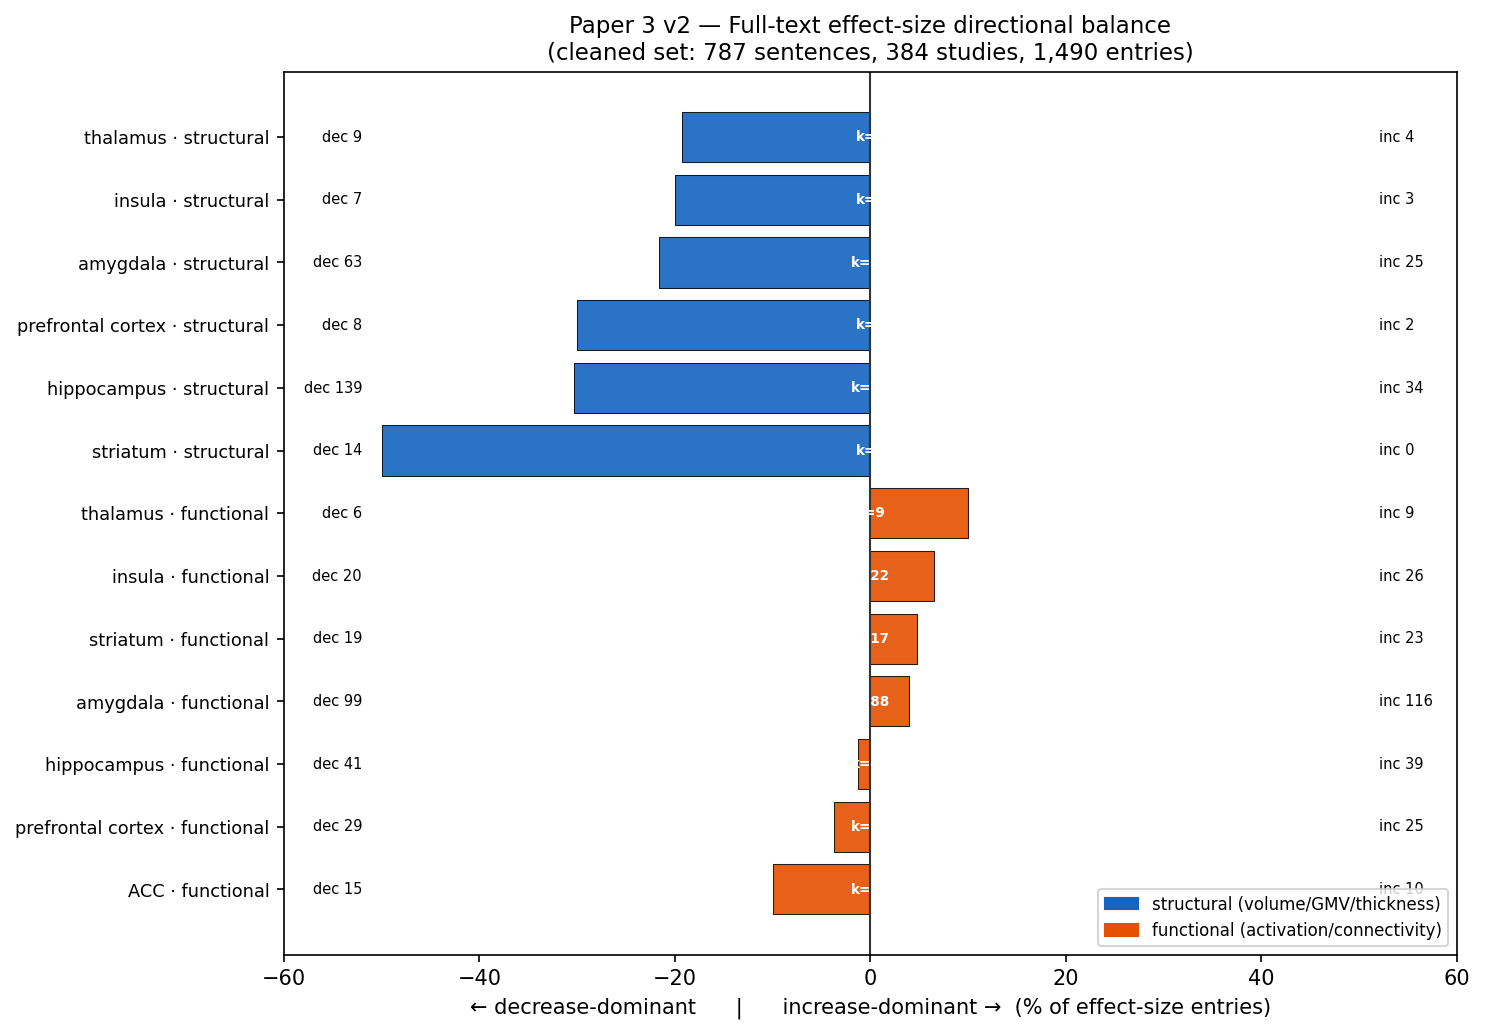
\includegraphics[width=\linewidth]{figures_v2/v2_fig1_directional_balance.png}
\caption{Full-text effect-size directional balance per brain region $\times$
metric class (cleaned set: 777 sentences, 380 studies, 1{,}006 entries in the
seven prioritised regions). Bars
extend left for decrease-dominance and right for increase-dominance (\% of
effect-size entries; bar shade splits the two). $k$ = number of studies
contributing entries to the cell, \emph{including} studies whose entries net to a
tie or null direction; $k$ therefore equals or exceeds the study-level
decrease+increase counts in Table~\ref{tab:dir} (which exclude ties/nulls---e.g.\
amygdala functional $k=87$ vs.\ $45+32=77$ non-tied studies). Structural metrics (blue) are decrease-dominant in every region (robust
at the study level for hippocampus and striatum); functional metrics (orange)
carry no significant directional signal. \textbf{Bar lengths are entry-level
proportions} (one study may contribute several entries, so bars can overstate
consensus through pseudoreplication); \textbf{every significance claim is made at
the study level} (one majority-vote direction per study) via the sign tests in
Table~\ref{tab:dir}, and bars are descriptive proportions of effect-size entries,
not pooled effects. The amygdala is the cautionary case: entry-level bars look
decrease-leaning, but the study-level test is non-significant ($p=0.13$).}
\label{fig:balance}
\end{figure}

\begin{table}[t]
\centering
\caption{Directional synthesis per brain region $\times$ metric class (cleaned
full-text effect sizes). The \textbf{study-level} sign test (majority-vote
direction per study) is the primary statistic; entry-level counts and $p$-values
are shown for completeness but are anti-conservative due to within-study
clustering. Sign test: exact two-sided binomial, ties/nulls excluded.}
\label{tab:dir}
\begin{tabular}{llrrr@{\hskip 12pt}rrr}
\toprule
 & & \multicolumn{3}{c}{Study-level} & \multicolumn{3}{c}{Entry-level} \\
\cmidrule(lr){3-5}\cmidrule(lr){6-8}
Region & Metric & Dec & Inc & $p$ & Dec & Inc & $p$ \\
\midrule
Hippocampus & structural & 55 & 12 & $\mathbf{1\times10^{-7}}$ & 135 & 34 & $1.9\times10^{-15}$ \\
Striatum & structural & 6 & 0 & $\mathbf{0.03}$ & 14 & 0 & $1.2\times10^{-4}$ \\
Amygdala & structural & 23 & 13 & 0.13 & 62 & 24 & $5.1\times10^{-5}$ \\
Amygdala & functional & 32 & 45 & 0.17 & 96 & 114 & 0.24 \\
Hippocampus & functional & 14 & 18 & 0.60 & 38 & 39 & 1.0 \\
Prefrontal cortex & functional & 18 & 13 & 0.47 & 29 & 25 & 0.68 \\
ACC & functional & 9 & 7 & 0.80 & 15 & 10 & 0.42 \\
Insula & functional & 10 & 12 & 0.83 & 20 & 26 & 0.46 \\
Striatum & functional & 7 & 7 & 1.0 & 19 & 23 & 0.64 \\
Thalamus & functional & 3 & 5 & 0.73 & 4 & 9 & 0.27 \\
Prefrontal cortex & structural & 4 & 0 & 0.13 & 8 & 2 & 0.11 \\
Thalamus & structural & 4 & 1 & 0.38 & 9 & 4 & 0.27 \\
Insula & structural & 4 & 3 & 1.0 & 7 & 3 & 0.34 \\
\bottomrule
\end{tabular}
\end{table}

\subsection{Structural measures are decrease-dominant}
Across structural metrics, every region leaned decrease-dominant at the entry
level (Figure~\ref{fig:balance}, Table~\ref{tab:dir}). At the
\emph{study level}---our primary unit---the structural decrease remained
significant for the hippocampus (55 vs.\ 12 studies; sign $p=1\times10^{-7}$) and
striatum (6 vs.\ 0; $p=0.03$), but \emph{not} for the amygdala (23 vs.\ 13;
$p=0.13$): the amygdala's entry-level significance ($p=5.1\times10^{-5}$) was driven
by within-study clustering and does not survive collapsing to one direction per
study. Prefrontal cortex, insula and thalamus were directionally consistent but
underpowered (all study-level $p>0.1$). The robust, study-level-significant
structural decrease is therefore \textbf{confined to the hippocampus}. A striatal
signal is also study-level significant (6 of 6 contributing studies report
decrease, $p=0.03$) but rests on too few studies to weight, and striatal
structural decrease is not part of the canonical stress phenotype; we treat it as
suggestive only. This is a narrower but more defensible claim than the
entry-level counts alone would suggest, and it matches the canonical
hippocampal-atrophy narrative using the studies' own reported effect sizes.

\subsection{Functional measures carry no consistent directional signal}
\textbf{No} functional contrast reached significance in either direction at the
study level (all $p>0.1$; Table~\ref{tab:dir}). The amygdala, often described as
showing increased reactivity under stress, was directionally flat---if anything
weakly increase-leaning (45 increase vs.\ 32 decrease studies, $p=0.17$), as was
the hippocampus (18 increase vs.\ 14 decrease, $p=0.60$). The functional signal is
therefore best described as directionally heterogeneous rather than as a coherent
increase.

\subsection{A structural--functional asymmetry, not a double dissociation}
Placing the two metric classes side by side (Figure~\ref{fig:balance}) reveals an
\emph{asymmetry} rather than a true double dissociation. The hippocampus shows
strong structural decrease (study-level $p=1\times10^{-7}$) with a near-balanced
functional profile ($p=0.60$); the amygdala shows neither a
study-significant structural decrease ($p=0.13$) nor a significant functional
increase ($p=0.17$). A genuine structural-down / functional-up dissociation would
require the functional contrast to reach significance in the increase direction,
which it does not in any region. The accurate statement is therefore that
\emph{structure decreases (robustly only in the hippocampus) while function
carries no consistent directional signal}---still informative, and still
consistent with the ``amygdala increases'' claim being weaker than the structural
decrease, but not a symmetric dissociation.

\begin{figure}[t]
\centering
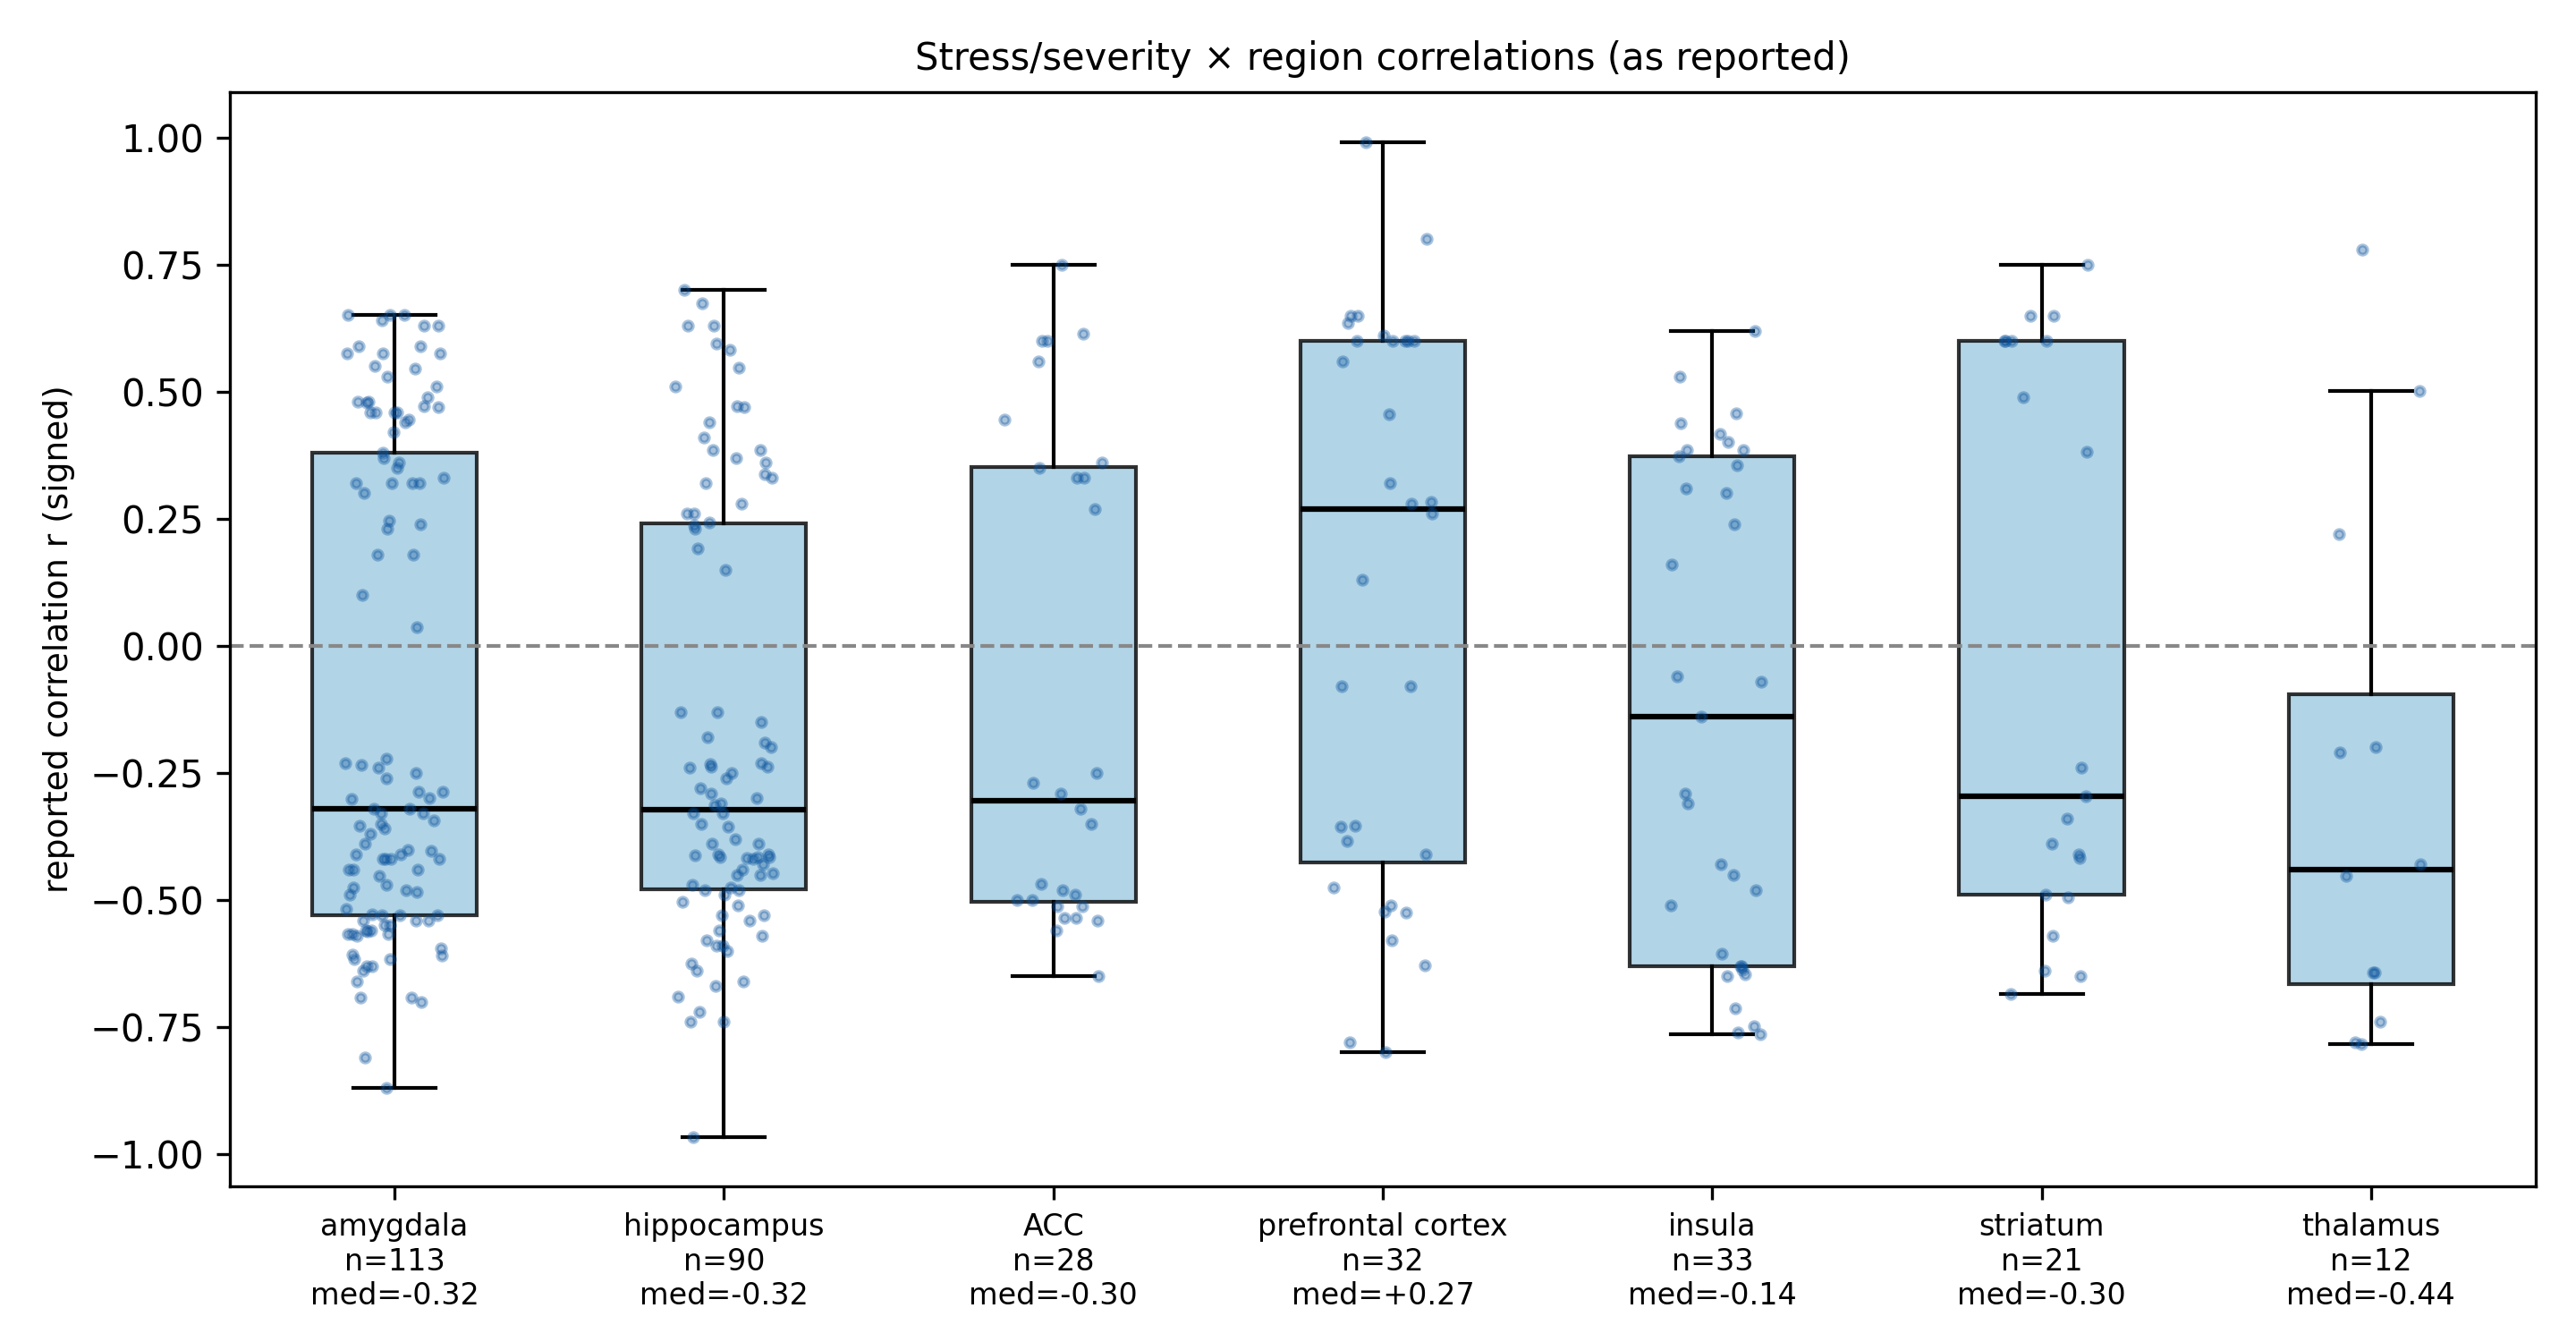
\includegraphics[width=0.85\linewidth]{figures_v2/v2_fig2_r_magnitude.png}
\caption{Distribution of $r$-type effect magnitudes per region (cleaned
full-text). Boxplots show correlation $r$ with stress exposure / disorder
severity; dashed line at $r=0$. Amygdala, hippocampus and ACC center near
$r\approx-0.3$ (moderate negative associations).}
\label{fig:rmag}
\end{figure}

\subsection{Correlation magnitudes as reported in the source studies}
Among $r$-type entries, correlations with stress exposure or disorder severity
clustered around $r\approx-0.30$ for the amygdala (median $-0.32$, $n=113$),
hippocampus ($-0.32$, $n=90$) and ACC ($-0.30$, $n=28$), indicating moderate
negative associations \emph{as reported} (Figure~\ref{fig:rmag})---but these
reported magnitudes are shown in \S3.7 to be inflated $\approx$4--6$\times$
relative to bias-free benchmarks. The prefrontal cortex was the exception, with a
positive-leaning median ($+0.27$, $n=32$), reflecting the heterogeneous and
task-dependent nature of prefrontal correlations in this literature.

\subsection{Extraction accuracy}
Applying the lexical \emph{silver} rule to all change-type (decrease/increase)
entries, 578 carried an unambiguous single-polarity cue and entered the
comparison; the model's mapped direction agreed with the silver label in 556/578
(\textbf{96.2\%}). The 22 disagreements were \emph{not} symmetric model errors:
manual inspection (the 22 cases listed de-identified in
\texttt{silver\_disagreements\_deidentified.csv}; source text via PMC) showed that 14
were \emph{silver-label} artifacts in which the cue word referred to the
comparison/control group (``higher gray matter in the control group''), to a
different region in a multi-region sentence, or formed a double negative (``less
negative connectivity''), and the model's patient-direction label was in fact
correct; a further 4 were source-contradictory sentences (a verbal ``greater''
alongside a negative reported Cohen's $d$) where the model followed the numeric
sign; only 4 were genuinely ambiguous. The 96.2\% agreement is therefore a
conservative \emph{lower} bound on direction accuracy, and the raw confusion
counts (19 model-decrease vs.\ lexical-increase, 3 the reverse) reflect the
prevalence of the ``greater-in-controls'' construction rather than a model bias
toward decrease. Because the silver label is derived from the same surface cues
the model keys on, this check applies only to lexically cued sentences.

On the \emph{LLM cross-check} of 50 hard-case-enriched sentences (\S2.6.1), the
second model \emph{agreed} with the original mapping on \textbf{90\%} (45/50);
agreement was \textbf{82\%} (14/17) on the hardest stratum (correlation-valence
items) and 93\% (14/15) on negation sentences. Because neither model is ground
truth, we report this as inter-model \emph{agreement}, not accuracy. The five
disagreements distribute as in Table~\ref{tab:crosscheck} (rows = original model
label, columns = cross-check label): the original model assigned ``decrease'' in
\emph{four} cases the cross-check did not echo (two $\to$ increase, two $\to$
null) and missed \emph{one} decrease the cross-check flagged (null $\to$
decrease). Read against the cross-check as a fallible reference, this raw pattern
leans, if anything, toward the model attributing decrease \emph{more} readily
than the cross-check, so the AI-vs-AI comparison \emph{alone does not exclude} a
mild decrease-favouring tendency---the failure mode that would inflate the
headline. We therefore read all five source sentences ourselves---the only
human-labelled step in the pipeline. Two of the four model-``decrease'' calls are
unambiguously correct on the text. In one, earlier age at first trauma exposure
was reported as associated with \emph{lower} [\textsuperscript{11}C]P943
5-HT\textsubscript{1B} receptor binding (BP\textsubscript{ND}) in striatal and
cingulate regions of PTSD patients \cite{murrough2011}; in the other, the
monozygotic cotwin with relatively \emph{higher} childhood cortisol showed
\emph{lower} amygdala--prefrontal connectivity \cite{burghy2016}. Both are
higher-stress$\to$lower-metric relationships whose sign the cross-check
mis-valenced. The other two are genuinely
ambiguous sentences that report \emph{both} directions at once (a putamen showing
``hyperactivation\dots\ and\dots\ hypoactivation''; a treatment-outcome
connectivity correlation), and neither concerns a headline region. The single
null$\to$decrease case is a structural-volume sentence (PTSD severity vs.\
hippocampal $d=-0.22$ \emph{and} amygdala $d=-0.12$, n.s.) on which the model was
the \emph{more conservative} of the two, mapping the non-significant effect as
null. Crucially, the headline failure mode---a true increase extracted as a
structural decrease---occurred in \textbf{none} of the five, and the only
structural disagreement had the model \emph{under}-calling, not over-calling,
decrease. The cross-check therefore provides no evidence of a decrease-inflating
extraction bias in the hippocampal signal, and this conclusion rests on a direct
reading of the five source sentences by the author, not on the cross-check model
alone. The larger residual uncertainty falls on the $r$-type
\emph{magnitude} distribution (correlation-valence agreement 82\%) rather than on
the directional sign tests. We stress that the two agreement checks (silver and
cross-check) are automated; only the five-sentence adjudication of disagreements
was performed by hand, and a full human audit of the larger extraction remains
future work.

\begin{table}[t]
\centering
\caption{Cross-check confusion matrix on the 50 hard-case-enriched sentences
(\S2.6.1). Rows = original model label, columns = independent cross-check label;
the diagonal (30+14+1 = 45) is inter-model agreement. The five off-diagonal
disagreements are examined sentence-by-sentence in \S3.6.}
\label{tab:crosscheck}
\begin{tabular}{lrrrr}
\toprule
model $\downarrow$ / cross-check $\rightarrow$ & decrease & increase & null & total \\
\midrule
decrease & 30 & 2 & 2 & 34 \\
increase & 0 & 14 & 0 & 14 \\
null & 1 & 0 & 1 & 2 \\
\midrule
total & 31 & 16 & 3 & 50 \\
\bottomrule
\end{tabular}
\end{table}

\subsection{Extracted magnitudes vs.\ individual-patient-data mega-analyses}
To external-validate our magnitude estimates, we compared them with the largest
individual-patient-data (IPD) mega-analyses of limbic structure, which are by
design free of publication bias. Converting our median correlations to Cohen's
$d$ ($d = 2r/\sqrt{1-r^2}$): hippocampus $r=-0.32 \to d\approx-0.68$; amygdala
$r=-0.32 \to d\approx-0.68$; ACC $r=-0.30 \to d\approx-0.63$. The corresponding
IPD estimates are markedly smaller: ENIGMA-PTSD reported hippocampus $d=-0.17$
and amygdala $d=-0.11$ (the latter not surviving multiple-comparison correction)
\cite{logue2018}, and ENIGMA-MDD reported hippocampus $d=-0.14$ (recurrent
$-0.17$) \cite{schmaal2016}. Two caveats sharpen this comparison. First, the
estimands differ: the IPD studies estimate a case--control \emph{group}
difference, whereas a sizeable share of our $r$-type entries are
\emph{severity} correlations within affected samples; these are not
interchangeable, so the ratio below should be read as an order-of-magnitude
discrepancy rather than a calibrated bias factor. Second, the cleanest
like-for-like benchmark is severity itself, and there the gap is starkest:
ENIGMA-MDD found \emph{no} association between symptom severity and regional
volume \cite{schmaal2016}, whereas our extracted severity correlations cluster
near $r\approx-0.3$---a qualitative discrepancy (null vs.\ moderate) that no
single multiplier captures. For the group-difference entries, our extracted
magnitudes exceed the unbiased benchmarks by $\approx$4--5$\times$ (hippocampus,
depending on which consortium estimate is used as the denominator) to
$\approx$6$\times$ (amygdala). Because our pipeline preferentially recovers the
\emph{reported}, typically significant, effect from each paper, these ratios are
if anything conservative lower bounds on the true reporting inflation. The
\emph{direction} of our synthesis therefore matches the gold standard, but its
\emph{magnitude} reflects the selective reporting of large, significant effects
in the publishable literature.

\section{Discussion}

The central result is two-sided. On \emph{direction}, full-text mining is
reassuring: stress-related structural decrease in the hippocampus is recovered
with study-level directional significance ($p=1\times10^{-7}$), matching both our
abstract-level counts and consortium mega-analyses. On \emph{magnitude}, it is
revisionist: the extracted correlations ($r\approx-0.3 \approx d\approx-0.68$)
overstate the unbiased mega-analytic effects ($d\approx-0.14$ to $-0.17$) by
4--6$\times$. The agreement between abstract-level and full-text \emph{counts}
therefore does not establish that the literature is unbiased---both inherit the
same upstream publication bias, which our magnitude comparison makes visible. The
contribution of this work is thus not merely to confirm a narrative, but to show
that LLM-scale mining can \emph{quantify the gap} between the published and the
unbiased estimate.

This matters methodologically, but the lesson is the opposite of a clean
validation. One might worry that abstract-level directional counting is an
artifact of how authors phrase abstracts. Full-text counts landing in the same
direction rules out a \emph{phrasing} artifact---but it cannot rule out
\emph{publication} bias, which acts on what is published at all rather than on
wording, and which abstracts and Results sections share equally. Our comparison
with IPD mega-analyses (\S3.7) makes this concrete: both abstract-level and
full-text estimates carry the same several-fold magnitude inflation relative to
the unbiased benchmark. The practical implication is that LLM-scale mining of
published text is a reliable instrument for \emph{direction} and for
\emph{quantifying the publication-bias gap}, but not a substitute for IPD pooling
when an unbiased magnitude is the goal. A second, sobering observation is that
the amygdala structural decrease---significant at the entry level but not at the
study level---would have been over-claimed by a sentence-level analysis;
study-level aggregation is therefore not a formality but a guard against
pseudoreplicated false positives.

\subsection{Limitations}
We are deliberately conservative in framing. First, \textbf{this is not a pooled
meta-analysis}: per-study sample sizes were extractable in only $\sim$6\% of
records, precluding inverse-variance weighting; we report directional sign tests
and magnitude distributions instead. Second, \textbf{mapping yield is moderate}
($\sim$43\% of stress-context candidate sentences produced a confident mapping);
unmapped sentences are dominated by null results and non-qualifying numbers, but
some true effects are missed, so counts are lower bounds. Third,
\textbf{pseudoreplication.} Extraction is at the sentence level, so a single
study can contribute multiple entries, violating the independence assumption of a
naïve sign test. We address this by making the study the primary unit
(majority-vote direction per study $\times$ region $\times$ metric; \S2.5); the
entry-level counts are retained only for transparency, and the amygdala result
illustrates that the distinction is material, not cosmetic. Residual
non-independence remains (studies share methods, populations, and field-level
priors), so even study-level significance is not equivalent to inverse-variance
pooling. Fourth, \textbf{vote-counting is a known-limited synthesis method}: it
ignores effect magnitude and per-study precision, and with underpowered
constituent studies it can converge on the wrong conclusion as study count grows
\cite{hedges1985,borenstein2009}. Our sign tests should be read as tests of
directional consistency in the published record, not as estimates of a pooled
effect. Fifth, \textbf{the magnitudes are conditioned on publication and
significance} (the ``winner's curse''); \S3.7 quantifies this as a 4--6$\times$
gap against IPD mega-analyses, and without per-study sample sizes we cannot
construct funnel plots or apply trim-and-fill, so the median $r$ values are
upper-leaning summaries of a selected sample, not bias-corrected population
effects. Sixth, \textbf{construct conflation}: the predictor ``stress exposure /
disorder severity'' pools heterogeneous constructs (chronic stress, PTSD, MDD,
early-life adversity, cortisol, perceived stress) whose relationships with
structure plausibly differ (e.g.\ ENIGMA-MDD found no severity--volume
association); the wide IQRs in Figure~\ref{fig:rmag} are consistent with this,
and stratified synthesis by exposure type is clear future work. Seventh, the
corpus is the PMC Open Access subset, which over-represents certain journals.
Eighth, \textbf{our validation establishes \emph{directional} accuracy, not
quantitative precision}: the silver and cross-check audits both score whether the
sign of the extracted effect is correct, and we make no claim that the pipeline
recovers the exact numeric value of each $r$ or $d$. Mis-parsed magnitudes
(e.g.\ a confidence-interval bound read as a point estimate, or a partial vs.\
zero-order correlation) would not be caught by a direction-only check; the
magnitude distributions in Figure~\ref{fig:rmag} should therefore be read as the
\emph{reported} values our parser recovered, with their own residual extraction
noise on top of the publication-bias inflation quantified in \S3.7. A numeric
audit of extracted magnitudes against hand-read values is clear future work.
These boundaries are exactly what separates this effect-size \emph{synthesis}
from a registered meta-analysis, which would require manual per-study
effect/sample-size curation on the prioritized regions.

\subsection{Conclusion}
Full-text effect-size synthesis across 380 studies recovers the \emph{direction}
of stress-related hippocampal structural decrease in the studies' own numbers,
but benchmarking against bias-free IPD mega-analyses shows the extracted
\emph{magnitudes} are inflated 4--6$\times$. LLM-scale mining of published text is
thus a reliable instrument for direction and for \emph{quantifying} the field's
publication bias---not for escaping it. We report the pipeline's direction
reliability honestly stratified by difficulty (96\% silver agreement on lexically
unambiguous sentences---a conservative lower bound---and 90\% inter-model
agreement on a hard subset enriched for negation and correlation-valence mapping;
the author's reading of the disagreement sentences found no decrease-inflating
error), its mapping yield ($\sim$43\%), and
the absence of usable sample sizes, so that the boundary between this synthesis
and a definitive meta-analysis is explicit.

\section*{Data and Code Availability}
\begin{itemize}
\item Complete list of all included studies (PMID, title, journal, year, PMC
ID): Supplementary Table~S1.
\item Source abstracts/full texts: retrievable from PubMed/PMC via the
identifiers in Supplementary Table~S1, under each article's respective license.
\item Extraction and synthesis code (\texttt{fulltext\_hybrid\_extract.py}, the
LLM-mapping runner, and the synthesis/sign-test scripts), the exact LLM prompt
(Appendix~A), and the de-identified LLM-mapped effect-size records are publicly
available at \url{https://github.com/shoo99/ai-drug-target} (directory
\texttt{paper3/}).
\end{itemize}

\section*{Companion preprint}
This study extends the abstract-level scoping review:
Kang B. (2026), \emph{Large-Scale Scoping Review of Chronic Stress-Induced Brain
Changes via LLM-Powered Extraction of 9,585 Studies}, Research Square,
\href{https://doi.org/10.21203/rs.3.rs-9884522/v1}{10.21203/rs.3.rs-9884522/v1}.

\section*{Acknowledgments}
LLM extraction was performed on a distributed CPU cluster (no GPU). Manuscript
preparation was assisted by Claude (Anthropic). The author takes full
responsibility for all scientific content.

\section*{Conflict of Interest}
The author declares no conflicts of interest.

\appendix
\section*{Appendix A. LLM extraction prompt (verbatim)}
Each candidate sentence was wrapped in the chat template
\texttt{<|im\_start|>user ... <|im\_end|><|im\_start|>assistant} with a
pre-closed \texttt{<think></think>} block (no-think mode) and the following
one-shot example and instruction:

\small
\begin{verbatim}
Example 1 (map: stress->region effect) —
Sentence: "Patients with PTSD showed reduced hippocampal volume vs controls
(Cohen's d=-0.45), and amygdala activation correlated with cortisol (r=0.38)."
Output: [{"brain_region":"hippocampus","metric":"volume","direction":"decrease",
"value":-0.45,"measure_type":"d"},{"brain_region":"amygdala",
"metric":"activation","direction":"positive_correlation","value":0.38,
"measure_type":"r"}]

[the candidate sentence + its regex-detected numbers are inserted here]

This sentence is FROM A CHRONIC-STRESS / STRESS-DISORDER STUDY (PTSD,
depression/MDD, early-life stress, trauma, high cortisol), so a brain-region
group difference or change reported here IS the stress/disorder effect — MAP IT.
Map a number when it quantifies a BRAIN REGION'S metric (volume, GMV, thickness,
activation, connectivity, FA, metabolite) as: patients vs controls, stressed vs
non-stressed, a within-patient change, or a correlation with a stress/severity
measure. direction = how the region's metric goes in the PATIENT/STRESSED/
higher-severity state (decrease/increase/positive_correlation/
negative_correlation/null). DO NOT map regression predictors (age, sex,
education, medication), task-performance correlations, scanner/coordinate
numbers, or protective-factor effects. Output ONLY a JSON array of
{brain_region, metric, direction, value, measure_type}; [] if none qualify.

Example 2 (nothing to map -> empty output) —
Sentence: "Reaction times were slower in the patient group (mean 612 vs 548 ms,
p=0.02), and head motion did not differ between groups (p=0.41)."
Output: []
(No brain-region metric is quantified: reaction time is task performance and head
motion is a nuisance covariate, so the correct output is the empty array.)
\end{verbatim}
\normalsize

\begin{thebibliography}{9}
\bibitem{kang2026scoping} Kang B. Large-Scale Scoping Review of Chronic
Stress-Induced Brain Changes via LLM-Powered Extraction of 9,585 Studies. {\it
Research Square} (2026). DOI: 10.21203/rs.3.rs-9884522/v1.
\bibitem{logue2018} Logue MW, van Rooij SJH, Dennis EL, et al. Smaller
Hippocampal Volume in Posttraumatic Stress Disorder: A Multisite ENIGMA-PGC
Study. {\it Biol Psychiatry} 2018;83(3):244--253.
doi:10.1016/j.biopsych.2017.09.006.
\bibitem{schmaal2016} Schmaal L, Veltman DJ, van Erp TGM, et al. Subcortical
brain alterations in major depressive disorder: findings from the ENIGMA Major
Depressive Disorder working group. {\it Mol Psychiatry} 2016;21:806--812.
doi:10.1038/mp.2015.69.
\bibitem{hedges1985} Hedges LV, Olkin I. {\it Statistical Methods for
Meta-Analysis}. Academic Press, 1985.
\bibitem{borenstein2009} Borenstein M, Hedges LV, Higgins JPT, Rothstein HR.
{\it Introduction to Meta-Analysis}. Wiley, 2009.
\bibitem{murrough2011} Murrough JW, Czermak C, Henry S, et al. The effect of
early trauma exposure on serotonin type 1B receptor expression revealed by
reduced selective radioligand binding. {\it Arch Gen Psychiatry}
2011;68(9):892--900. PMID:21893657.
\bibitem{burghy2016} Burghy CA, Fox ME, Cornejo MD, et al. Experience-driven
differences in childhood cortisol predict affect-relevant brain function and
coping in adolescent monozygotic twins. {\it Sci Rep} 2016;6:37081.
PMID:27872489.
\end{thebibliography}

\end{document}
